\documentclass{beamer}
\usepackage{color}
\usepackage{xcolor}
\usepackage[backend=biber]{biblatex}
\usepackage{tikz}
\setbeamertemplate{bibliography item}{\insertbiblabel}

\RequirePackage{currfile} 
\setbeamertemplate{caption}[numbered]

\usetheme{Frankfurt}
%\usecolortheme{whale}

\addbibresource{main.bib}

%--------Stuff for Compartment/Blocks-----%
\usetikzlibrary{arrows}
\tikzstyle{block} = [rectangle, draw, text width = 1.5em, text centered, minimum height = 1.5em]
\tikzstyle{line} = [thick, ->, >= stealth]
\tikzstyle{noBlock} = [rectangle, draw = none]

%\logo{
\includegraphics[width = 0.5 in]{Figures/epscor.jpeg}}

\definecolor{maincol}{HTML}{4B778D}
\definecolor{secondcol}{RGB}{75,119,141}
\definecolor{thirdcol}{RGB}{40,181,181}
\setbeamercolor{palette primary}{bg = maincol, fg=white}
\setbeamercolor{palette secondary}{bg = secondcol, fg=white}
\setbeamercolor{palette tertiary}{bg=thirdcol, fg=white}
\setbeamercolor{palette quaternary}{bg = thirdcol, fg=white}
\setbeamercolor{structure}{fg=maincol}
\setbeamercolor{section in toc}{fg=maincol} 
\setbeamercolor{subsection in head/foot}{bg=maincol, fg=white}

%%--------------- Title Slide ------------------------------
\title[]{Model of Guam's Coral Reef Change}
\subtitle{Coral Reefsearchers}
\author{Aaron Bumagat, Michelle Luces, Henry Song }
\institute{University of Guam}
\date{\today} 


\begin{document}
\frame{\titlepage}

\AtBeginSection[]{}
\begin{frame}<Beamer>
\frametitle{}
\setcounter{tocdepth}{2}
\tableofcontents{currentsection, sections = \thesection}
\setcounter{tocdepth}{1}
\end{frame}

%%------------------Table of Contents---------------------------
\begin{frame}{Table of Contents}
\tableofcontents
\end{frame}

%%-----------------------Introduction----------------------------
\section{Introduction}
\begin{frame}{Introduction}
\begin{itemize}
    \item General Question: How will Guam's reef ecosystem change over the coming decades?
\end{itemize}
\begin{figure}
    \centering
    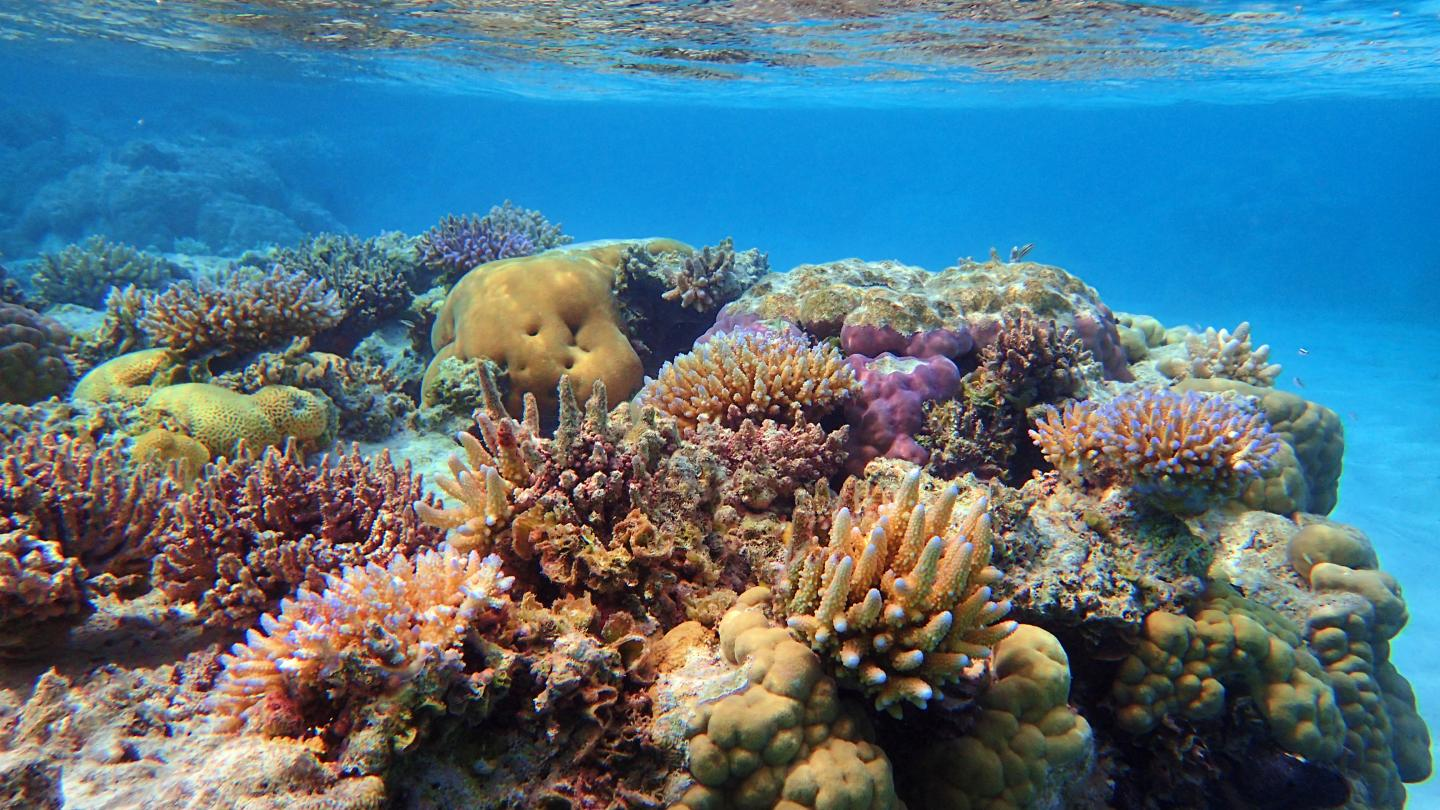
\includegraphics[width=0.6\textwidth]{Figures/coral_picture.jpg}
    %\caption{Caption}
    %\label{fig:my_label}
\end{figure}
\end{frame}

%%--------------------------Background--------------------------
\section{Background}
% \begin{frame}{Background}
%     \begin{itemize}
%         \item Coral Reefs are large underwater structures composed of the skeletons of colonial marine invertebrates known as coral$^\cite{ross}$.
%     \end{itemize}
% \end{frame}
% \begin{frame}{Background}
%     \begin{itemize}
%         \item Coral Reefs are large underwater structures composed of the skeletons of colonial marine invertebrates known as coral$^\cite{ross}$.
%         \item Climate change is a leading factor for the cause of coral bleaching/death.
%     \end{itemize}
% \end{frame}
% \begin{frame}{Background}
%     \begin{itemize}
%         \item Coral Reefs are large underwater structures composed of the skeletons of colonial marine invertebrates known as coral$^\cite{ross}$.
%         \item Climate change is a leading factor for the cause of coral bleaching/death.
%         \item Overfishing, temperature changes, and resiliency of coral reef species are factors when it comes to the changes in a reef ecosystem.
%     \end{itemize}
% \end{frame}
\begin{frame}{Background}
    \begin{itemize}
        \item<1-> Coral Reefs are large underwater structures composed of the skeletons of colonial marine invertebrates known as coral$^\cite{ross}$.
        \item<2-> Climate change is a leading factor for the cause of coral bleaching/death.
        \item<3-> Other factors that contribute to changes in a reef ecosystem are overfishing, temperature changes, and coral reef resilience.
        \item<4-> According to the 2008 State of the Coral Reef Ecosystems of Guam report, Guam’s coral reef resources are both economically and culturally important, providing numerous goods and services for the residents of Guam, including cultural/traditional use, tourism, recreation, fisheries, and shoreline/infrastructure protection$^\cite{guamwebsite}$.
    \end{itemize}
\end{frame}


%%------------------------Literature Review----------------
\section{Literature Review}
\begin{frame}{Literature Review}
Articles covered:
\begin{itemize}
    \item Assessing relative resilience potential of coral reefs to inform management$^\cite{assesing_relative}$
    \item Prioritizing Key Resilience Indicators to Support Coral Reef Management in a Changing Climate$^\cite{prioritize}$
    \item Model of coral population response to accelerated bleaching and mass mortality in a changing climate$^\cite{Riegl_Purkis_Model}$
    \item Mathematical Analysis of Coral Reef Models$^\cite{mathanalysis}$
\end{itemize}
\end{frame}

\subsection{Assessing relative resilience potential of coral reefs to inform management}
\begin{frame}{Assessing relative resilience potential of coral reefs to inform management}
    \begin{block}{Summary}
        \small{This research discusses ecological resilience as a essential part of resilience-based management (RBM) and the use of such assessments to explain resilience potentials of coral reefs in the Northern Mariana Islands (CNMI).}
    \end{block}
    Why is this article important?
    \begin{itemize}
        \item Explores and elaborates on factors affecting coral resilience.
        \item Acts as a guide to implement ecological resilience assessments.
        \item Analyzes inter-island and intra-island connectivity.
    \end{itemize}
\end{frame}

\subsection{Prioritizing Key Resilience Indicators to Support Coral Reef Management in a Changing Climate}
\begin{frame}{Prioritizing Key Resilience Indicators to Support Coral Reef Management in a Changing Climate}
    \begin{block}{Summary}
        Empirical selection criteria was created in order to prioritize coral reef management.
    \end{block}
    Why is this article important?
    \begin{itemize}
        \item Provides data from certified scientists when it comes to resilience of coral reef.
            \begin{itemize}
                \item Can be used to see which will be focused on when creating our parameters.
            \end{itemize}
    \end{itemize}
\end{frame}

%\begin{frame}{Prioritizing Key Resilience Indicators to Support Coral Reef Management in a Changing Climate Cont.}
%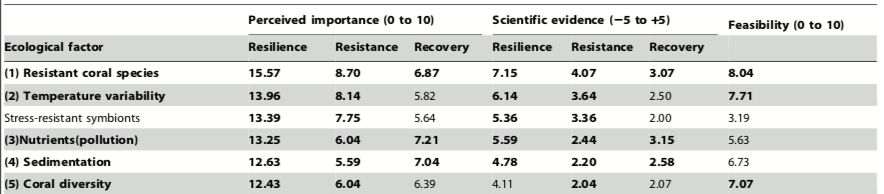
\includegraphics[width = 4.3 in. , height = 1.7 in.]{Figures/Resilience Data.png}
%\end{frame}

\subsection{Model of coral population response to accelerated bleaching and mass
mortality in a changing climate}
\begin{frame}{Model of coral population response to accelerated bleaching and mass
mortality in a changing climate}
    \begin{block}{Summary}
        Researchers studied coral populations located within the Arabian Peninsula. The study primarily focused on the Porites and \textit{Acropora} species of coral. The researchers found that coral populations can survive more extreme conditions.
    \end{block}
\end{frame}

\begin{frame}{Model of coral population response to accelerated bleaching and mass
mortality in a changing climate (Cont.)}
    Why is this article important?
    \begin{itemize}
        \item Methods used include a system of differential equations.
        \item It implements a compartment model to illustrate the relationships.
        \item It uses the Lotka-Volterra model to simulate a predator prey relationship between \textit{Acropora} as the dominant species and others as the recessive species.
        \begin{itemize}
            \item Incorporates ideas of Game Theory into methods.
        \end{itemize}
    \end{itemize}
\end{frame}

\subsection{Mathematical Analysis of Coral Reef Models}
\begin{frame}{Mathematical Analysis of Coral Reef Models}
    \begin{block}{Summary}
        This research analyzes grazing in response to threatened coral reef systems. Specifically, this model is focused on the impact of different grazing intensities and their influences on coral-algae interactions. Results provided from this research can provide insight on how to revitalize unhealthy reefs.
    \end{block}
\end{frame}

\begin{frame}{Mathematical Analysis of Coral Reef Models (Cont.)}
    Why is this article important?
    \begin{itemize}
        \item The authors used ordinary differential equations (ODE) and delay differential equations (DDE) to model coral reefs.
        \item Discusses about the stability of three different states: extinction state, macroalgae-only state, and coral-only state.
        \item  The mathematical results can help answer how to reverse the unhealthy reefs to a healthy status by knowing how overfishing affects our reefs.
    \end{itemize}
\end{frame}

%%------------------------------------------------------


%%-----------------------------Plan-------------------------
\section{Plans}
\begin{frame}{Compartment Model}
\begin{center}
    \begin{tikzpicture}{node distance = 1cm, auto}
        \node (S) [block] {S}; 
        \node (E) [block, right of = S, node distance = 3 cm] {E};
        \node (I) [block, right of = E, node distance = 3 cm] {I};
        \node (R) [block, right of = I, node distance = 3 cm] {R};
        \node (H) [block, below of = E, node distance = 2 cm] {H};
        \draw[line] (S) --node[above]{} (E);
        \draw[line] (H) --node[above]{} (S);
        \draw[line] (E) --node[above]{} (I);
        %\draw[line] (H) --node[above]{} (I);
        \draw[line] (I) --node[above]{} (R);
    \end{tikzpicture}
\end{center}
\begin{block}{Compartments }
    \begin{itemize}
    \item $S$: all susceptible corals
    \item $E$: our exposed corals
    \item $I$: our infected corals
    \item $R$: our recovered corals
    \item $H$: human factors potentially affecting coral reefs
\end{itemize}
\end{block}
%\begin{itemize}
    %\item Compartment $S$ represents all susceptible corals.
    %\item Compartment $H$ represents the human factors potentially affecting coral reefs.
    %\item Compartment $E$ represents our exposed corals.
    %\item Compartment $I$ represents our infected corals.
    %\item Compartment $R$ represents our recovered corals.
%\end{itemize}
\end{frame}

\begin{frame}{Plans}
    \begin{itemize}
        \item Specific ideas:
        \begin{itemize}
            \item How will a specific coral species change throughout the upcoming decades on Guam?
            \item Select a representative species of average resiliency (specifically on Guam) and examine how it will change over time through climate changes.
        \end{itemize}
        %\item Continue to digest articles and literature relevant to our research.
        \item Establish our methodology and mathematical model in order finalize our compartment model and to answer our question.
        \item Application of Game Theory (specifically education game theory).
    \end{itemize}
\end{frame}

%----------------------------------------------------


%---------------------Conclusion---------------------
%\section{Conclusion}
%\begin{frame}{Conclusion}
    %Type conclusion here
%\end{frame}


\begin{frame}
    \Huge{Questions?}
\end{frame}

\section{Q \& A}


%%-------------------------Acknowledgements----------------
\section{Acknowledgements}
\begin{frame}{Acknowledgements}
    \begin{center}
        Support for the Young Scholars Research Experience in Mathematics (YSREM)  is through the MAA Tensor SUMMA Program. Support for the MAA National Research Experience for Undergraduates Program (NREUP) is provided by the National Science Foundation (Grant Number DMS-1950644). Support for the NSF EPSCoR project, Guam Ecosystems Collaboratorium for Corals and Oceans (GECCO) is provided by the National Science Foundation (Grant Number DMS-1946352). \\
    \vspace{.2cm}
    \small{Special thanks to Dr. Bastian Bentlage, our faculty mentors (Dr. JaeYong Choi, Dr. HyunJu Oh, \& Dr. Leslie Aquino), and our Research Assistants (Jaron Bautista \& Regina-Mae Dominguez).}
    
    \begin{figure}
        
\includegraphics[width = 0.20\textwidth]{Figures/MAA_logo_PMS286.jpg}
        \label{MAA}
        
\includegraphics[width = 0.12\textwidth]{Figures/NSF_4-Color_bitmap_Logo.png}
        \label{NSF}
        % 
\includegraphics[width = 0.20\textwidth]{Figures/GECCO.png}
        % \label{gecco}
        
\includegraphics[width = 0.12\textwidth]{Figures/epscor.jpeg}
        \label{epscor}
        
\includegraphics[width = 0.20\textwidth]{Figures/UOG-horizontal.png}
        \label{uog}
    \end{figure}
    \end{center}
\end{frame}




%%----------------------Bibliography-------------------
\section{Bibliography}
\begin{frame}[allowframebreaks]{Bibliography}
    \tiny{\printbibliography}
\end{frame}


%%---------------Thank you/Questions----------------------

\begin{frame}
    \Huge{Thank you!}
\end{frame}


\end{document}